\documentclass[conference]{IEEEtran}
\IEEEoverridecommandlockouts

\usepackage[utf8]{inputenc}
\usepackage[T1]{fontenc}
\usepackage{cite}
\usepackage{amsmath,amssymb,amsfonts}
\usepackage{algorithmic}
\usepackage{graphicx}
\usepackage{textcomp}
\usepackage{xcolor}
\usepackage{url}

\def\BibTeX{{\rm B\kern-.05em{\sc i\kern-.025em b}\kern-.08em
    T\kern-.1667em\lower.7ex\hbox{E}\kern-.125emX}}

\begin{document}

% Título propuesto a partir del contenido del documento fuente.
\title{Predicción de Mortalidad Hospitalaria mediante Machine Learning con el Dataset SUPPORT}

\author{
\IEEEauthorblockN{1\textsuperscript{st} Joaquin Geronimo Arriaga Cosio}
\IEEEauthorblockA{
\textit{Ciencia de la Computación} \\
\textit{Universidad de Ingeniería y Tecnología (UTEC)} \\
Lima, Perú
}
\and

\IEEEauthorblockN{2\textsuperscript{nd} Marialejandra Bautista Gastelo}
\IEEEauthorblockA{
\textit{Ciencia de la Computación} \\
\textit{Universidad de Ingeniería y Tecnología (UTEC)} \\
Lima, Perú
}
\and

\IEEEauthorblockN{\makebox[\linewidth][c]{3\textsuperscript{rd} Elizabeth Huaman Santillan}}
\IEEEauthorblockA{\parbox{\linewidth}{\centering
\textit{Ciencia de la Computación} \\
\textit{Universidad de Ingeniería y Tecnología (UTEC)} \\
Lima, Perú
}}
}

\maketitle

\begin{abstract}
En este proyecto se propone desarrollar un modelo de Machine Learning para predecir la mortalidad hospitalaria en pacientes con enfermedades graves utilizando variables demográficas, clínicas y fisiológicas. Para el análisis se utilizó el dataset SUPPORT, que contiene 9105 observaciones y 47 variables, considerando como variable objetivo \texttt{hospdead}, donde 1 representa el fallecimiento del paciente durante la hospitalización y 0 indica que el paciente sobrevivió. Como parte del análisis exploratorio se evaluaron los valores faltantes, la distribución de la variable objetivo, las diferencias en variables fisiológicas entre pacientes sobrevivientes y fallecidos, la correlación entre variables numéricas y la presencia de valores atípicos. También se identificaron variables que podrían generar data leakage, como puntuaciones de severidad y estimaciones pronósticas previas, por lo que no fueron consideradas como predictores principales. Este análisis permite establecer una base para las siguientes etapas de preprocesamiento y modelado, donde se evaluará si las variables fisiológicas permiten obtener una mejor capacidad predictiva que un modelo basado únicamente en variables demográficas.
\end{abstract}

\begin{IEEEkeywords}
Machine Learning, mortalidad hospitalaria, SUPPORT, variables fisiológicas, clasificación, análisis exploratorio de datos.
\end{IEEEkeywords}

\section{Introducción y formulación del problema}
La estimación temprana del riesgo de mortalidad en pacientes hospitalizados es un problema central en la medicina crítica, ya que orienta decisiones clínicas, la comunicación con pacientes y familiares, y la asignación de recursos hospitalarios. El estudio SUPPORT fue diseñado precisamente para mejorar la toma de decisiones en el cuidado de pacientes con enfermedades graves, mediante la construcción de modelos pronósticos objetivos basados en variables fisiológicas y clínicas \cite{knaus1995}.

En este proyecto se plantea la siguiente tarea de Machine Learning: dado un conjunto de variables demográficas, de comorbilidad y fisiológicas registradas durante los primeros días de hospitalización, predecir si el paciente fallecerá durante la hospitalización (variable \texttt{hospdead}).

\textbf{Pregunta de investigación:} ¿En qué medida las variables fisiológicas registradas el día 3 de hospitalización permiten predecir la mortalidad hospitalaria con mayor capacidad discriminativa que las variables puramente demográficas (edad, sexo, ingreso)?

\textbf{Hipótesis:} se espera que los modelos que incorporan variables fisiológicas (por ejemplo, score APACHE-like, presión arterial media, frecuencia respiratoria) superen sustancialmente a un baseline demográfico, dado que reflejan directamente la severidad clínica del paciente.

\section{Datos y Análisis Exploratorio de Datos (EDA)}

\subsection{Descripción del dataset}
Se utilizó el dataset \textit{support2}, correspondiente al estudio SUPPORT (Study to Understand Prognoses Preferences Outcomes and Risks of Treatment) \cite{supportdata}. El conjunto contiene 9105 observaciones correspondientes a pacientes hospitalizados con enfermedades graves y un total de 47 variables de naturaleza demográfica, clínica, fisiológica y pronóstica.

Cada observación representa a un paciente. Entre las variables disponibles se encuentran edad, sexo, raza, diagnóstico principal, número de comorbilidades y diferentes mediciones fisiológicas, como presión arterial media, frecuencia cardíaca, frecuencia respiratoria, temperatura, razón PaO$_2$/FiO$_2$, albúmina, bilirrubina, creatinina, sodio, glucosa, BUN y recuento de leucocitos.

La variable objetivo seleccionada fue \texttt{hospdead}, de naturaleza binaria, donde el valor 1 representa el fallecimiento del paciente durante la hospitalización y el valor 0 indica que el paciente sobrevivió al periodo hospitalario.

\subsection{Análisis de valores faltantes}
Como parte del análisis inicial de calidad de datos, se cuantificó la cantidad y proporción de valores faltantes para cada variable. Este análisis es especialmente relevante debido a que varias variables fisiológicas y clínicas presentan observaciones incompletas.

Se calculó el porcentaje de datos faltantes respecto del total de 9105 pacientes y se ordenaron las variables de mayor a menor proporción de ausencia. Esto permite identificar aquellas características cuya utilización puede requerir posteriormente estrategias específicas de imputación o, en casos de ausencia excesiva, evaluar su conveniencia dentro del conjunto de predictores.

En esta etapa no se realizó todavía la imputación definitiva de los valores faltantes, ya que modificar los datos antes de completar el análisis exploratorio podría alterar las distribuciones originales. Las estrategias de imputación serán incorporadas posteriormente durante la etapa de preprocesamiento.

\subsection{Prevención de data leakage}
Antes de analizar las relaciones entre los predictores y la mortalidad hospitalaria se identificaron variables que podrían introducir fuga de información o incorporar estimaciones pronósticas externas al modelo que se desea desarrollar.

Se consideraron para exclusión \texttt{sps}, \texttt{aps}, \texttt{surv2m}, \texttt{surv6m}, \texttt{prg2m}, \texttt{prg6m}, \texttt{dnr} y \texttt{dnrday}. Las variables \texttt{sps} y \texttt{aps} corresponden a puntuaciones de severidad fisiológica obtenidas mediante modelos previamente desarrollados; \texttt{surv2m} y \texttt{surv6m} representan estimaciones previas de supervivencia; \texttt{prg2m} y \texttt{prg6m} contienen estimaciones pronósticas realizadas por el médico; mientras que \texttt{dnr} y \texttt{dnrday} contienen información relacionada con órdenes de no reanimación.

Estas variables no serán utilizadas como predictores principales durante el análisis y modelado, con el objetivo de evaluar la capacidad predictiva de las características clínicas y fisiológicas originales y reducir el riesgo de obtener estimaciones artificialmente optimistas.

\subsection{Distribución de la variable objetivo}
Se analizó la distribución de la variable objetivo \texttt{hospdead} para determinar la proporción de pacientes que sobrevivieron y fallecieron durante la hospitalización. Se calcularon las frecuencias absolutas y relativas de ambas clases y se representaron mediante un gráfico de barras.

El análisis permitió evaluar la presencia de un posible desbalance entre clases, aspecto relevante para la posterior selección de métricas de evaluación. En caso de existir una diferencia considerable entre el número de sobrevivientes y fallecidos, métricas como la exactitud global podrían no representar adecuadamente el desempeño del modelo, por lo que será necesario considerar métricas complementarias como sensibilidad, precisión, F1-score o AUC-ROC.

Los resultados obtenidos fueron de [N0] pacientes sobrevivientes ([P0]\%) y [N1] pacientes fallecidos ([P1]\%).

\begin{figure}[htbp]
\centering
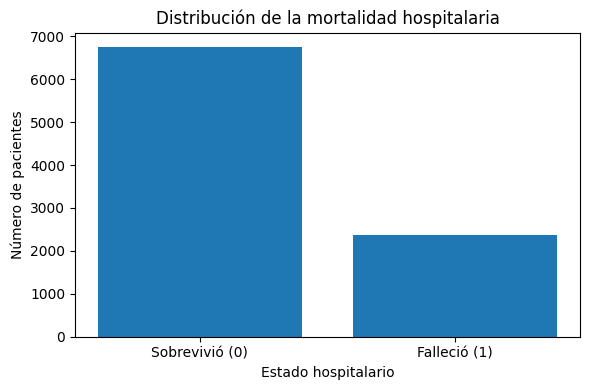
\includegraphics[width=\columnwidth]{figures/image7.png}
\caption{Distribución de la mortalidad hospitalaria.}
\label{fig:mortalidad}
\end{figure}

\subsection{Análisis de variables fisiológicas según mortalidad}
Con el objetivo de explorar posibles diferencias clínicas entre pacientes sobrevivientes y fallecidos, se analizaron las distribuciones de las principales variables fisiológicas disponibles en el dataset.

Se incluyeron presión arterial media (\texttt{meanbp}), frecuencia cardíaca (\texttt{hrt}), frecuencia respiratoria (\texttt{resp}), temperatura (\texttt{temp}), razón PaO$_2$/FiO$_2$ (\texttt{pafi}), albúmina (\texttt{alb}), bilirrubina (\texttt{bili}), creatinina (\texttt{crea}), sodio (\texttt{sod}), pH, glucosa (\texttt{glucose}), BUN (\texttt{bun}), recuento de leucocitos (\texttt{wblc}) y producción urinaria (\texttt{urine}).

Para cada variable se calcularon la media, mediana y desviación estándar de forma independiente para pacientes con \texttt{hospdead = 0} y \texttt{hospdead = 1}. Adicionalmente, se utilizaron diagramas de caja para visualizar diferencias en las distribuciones de algunas variables clínicas representativas.

Este análisis es de carácter exploratorio y permite identificar características potencialmente asociadas con la mortalidad hospitalaria, sin asumir todavía que dichas diferencias impliquen una relación causal o una capacidad predictiva independiente.

\begin{figure}[htbp]
\centering
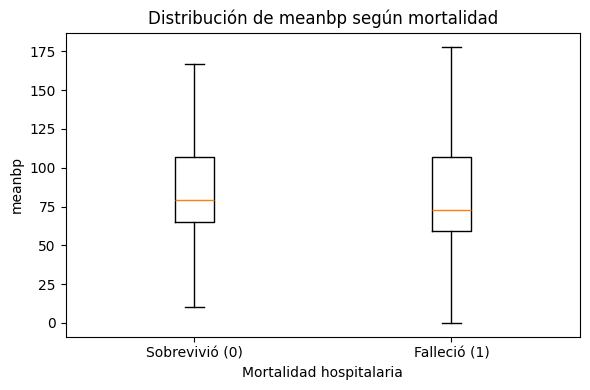
\includegraphics[width=\columnwidth]{figures/image3.png}
\caption{Distribución de \texttt{meanbp} según mortalidad hospitalaria.}
\label{fig:meanbp}
\end{figure}

\begin{figure}[htbp]
\centering
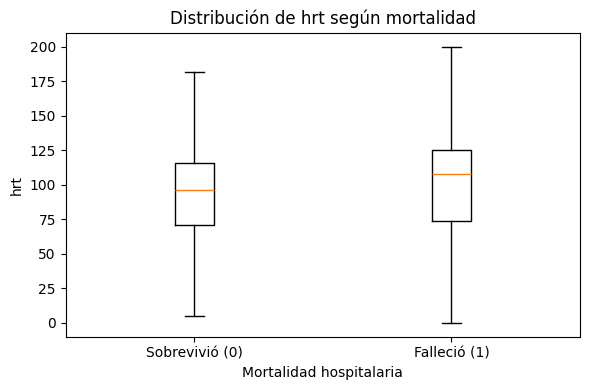
\includegraphics[width=\columnwidth]{figures/image4.png}
\caption{Distribución de \texttt{hrt} según mortalidad hospitalaria.}
\label{fig:hrt}
\end{figure}

\begin{figure}[htbp]
\centering
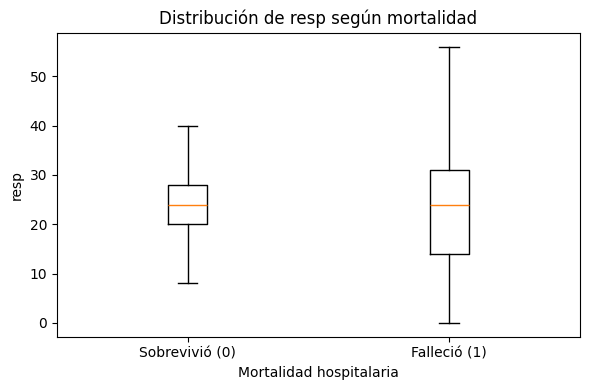
\includegraphics[width=\columnwidth]{figures/image8.png}
\caption{Distribución de \texttt{resp} según mortalidad hospitalaria.}
\label{fig:resp}
\end{figure}

\begin{figure}[htbp]
\centering
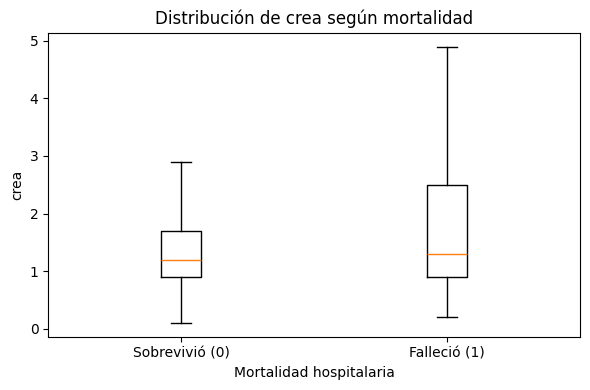
\includegraphics[width=\columnwidth]{figures/image6.png}
\caption{Distribución de \texttt{crea} según mortalidad hospitalaria.}
\label{fig:crea}
\end{figure}

\begin{figure}[htbp]
\centering
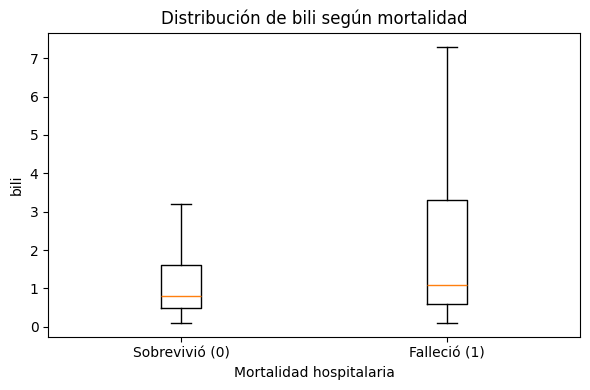
\includegraphics[width=\columnwidth]{figures/image5.png}
\caption{Distribución de \texttt{bili} según mortalidad hospitalaria.}
\label{fig:bili}
\end{figure}

\begin{figure}[htbp]
\centering
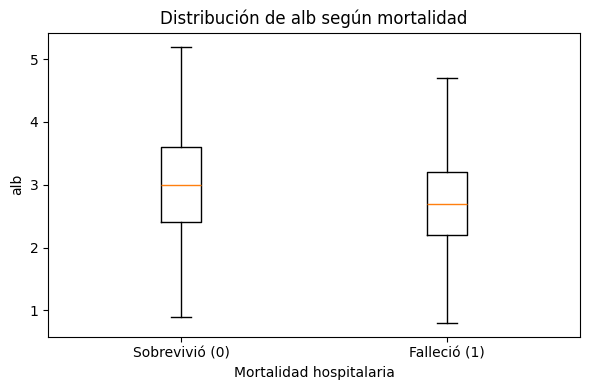
\includegraphics[width=\columnwidth]{figures/image1.png}
\caption{Distribución de \texttt{alb} según mortalidad hospitalaria.}
\label{fig:alb}
\end{figure}

\subsection{Análisis de correlación entre variables numéricas}
Se evaluó la asociación lineal entre las principales variables numéricas y la mortalidad hospitalaria mediante el coeficiente de correlación de Pearson. Para facilitar la interpretación, se analizaron específicamente las correlaciones de cada característica con la variable objetivo \texttt{hospdead}, ordenándolas según su magnitud absoluta.

Este análisis permite identificar qué variables presentan una mayor asociación lineal con el desenlace hospitalario. Sin embargo, una correlación baja no implica necesariamente una baja utilidad predictiva, ya que pueden existir relaciones no lineales que posteriormente sean identificadas por los modelos de Machine Learning.

\begin{figure}[htbp]
\centering
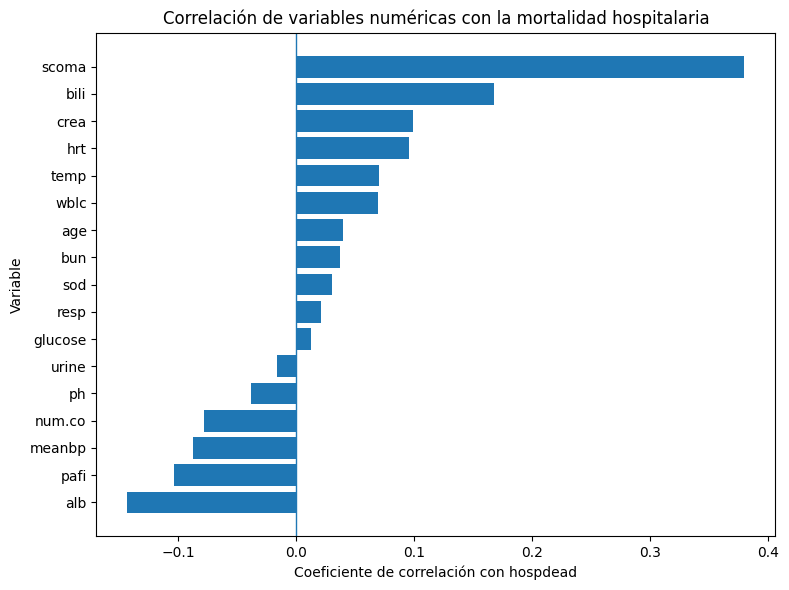
\includegraphics[width=\columnwidth]{figures/image2.png}
\caption{Correlación de variables numéricas con la mortalidad hospitalaria.}
\label{fig:correlacion}
\end{figure}

\subsection{Identificación de valores atípicos}
Se evaluó la presencia de valores atípicos en las principales variables fisiológicas mediante el criterio del rango intercuartílico (IQR). Para cada variable se calcularon el primer cuartil (Q1), tercer cuartil (Q3) y el rango intercuartílico, definiendo como potenciales valores atípicos aquellas observaciones inferiores a $Q1 - 1.5\cdot IQR$ o superiores a $Q3 + 1.5\cdot IQR$.

Se calculó tanto el número como el porcentaje de observaciones identificadas como atípicas para cada variable. Sin embargo, estos valores no fueron eliminados automáticamente. Debido a que el dataset corresponde a pacientes con enfermedades graves, mediciones fisiológicas extremas pueden representar condiciones clínicas reales y no necesariamente errores de registro.

Por esta razón, el análisis de valores atípicos se utiliza en esta etapa principalmente para caracterizar la distribución de los datos. Cualquier tratamiento posterior deberá considerar tanto criterios estadísticos como la plausibilidad clínica de las observaciones.

\subsection{Principales hallazgos del EDA}
El análisis exploratorio permitió caracterizar la estructura y calidad del dataset SUPPORT antes de realizar cualquier procedimiento de modelado. El conjunto presenta una combinación de variables demográficas, diagnósticas y fisiológicas, así como una proporción considerable de valores faltantes en determinadas características.

La evaluación de \texttt{hospdead} permitió determinar la distribución de las dos clases y establecer si será necesario considerar estrategias específicas frente a un eventual desbalance. Por otra parte, la comparación de variables fisiológicas entre pacientes sobrevivientes y fallecidos permitió identificar diferencias exploratorias en determinados parámetros clínicos.

El análisis de correlación permitió estudiar asociaciones lineales entre variables y detectar posibles redundancias, mientras que el análisis basado en el rango intercuartílico identificó la presencia de valores extremos en diferentes características fisiológicas. Debido a la naturaleza clínica de la población estudiada, estos valores no serán considerados automáticamente errores.

Finalmente, la identificación previa de variables con riesgo de data leakage permite establecer un conjunto de características más adecuado para las etapas posteriores del proyecto. Los resultados obtenidos durante este EDA servirán de base para definir las estrategias de imputación, codificación, escalamiento y selección de variables que serán implementadas durante la etapa de preprocesamiento.
\subsection{Disponibilidad del código}
El código, notebooks y recursos necesarios para reproducir los análisis y experimentos de este trabajo se encuentran disponibles en el siguiente repositorio público:
\url{https://github.com/VannaNotGianna/Prediccion_mortalidad_hospitalaria_ml}

\begin{thebibliography}{00}
\bibitem{knaus1995}
W. A. Knaus, F. E. Harrell, J. Lynn, et al., ``The SUPPORT prognostic model: Objective estimates of survival for seriously ill hospitalized adults,'' \textit{Annals of Internal Medicine}, vol. 122, pp. 191--203, 1995.

\bibitem{supportdata}
Vanderbilt University Department of Biostatistics, ``SUPPORT Datasets.'' [Online]. Available: \url{https://hbiostat.org/data/repo/supportdesc}
\end{thebibliography}

\end{document}
